\chapter{Clustered Attractor Networks}
\label{ch:clustered-attractor-networks}

\textit{A clustered network turns recurrent excitation into a memory of which
cell assemblies are active. In E-clustered networks with homogeneous
inhibition, switching between active-cluster patterns is naturally interpreted
as finite-size noise moving the system among metastable attractors.}

% ============================================================
\section{Cell Assemblies as Structured Recurrence}
\label{sec:cell-assemblies}
% ============================================================

The balanced random network of Chapter~\ref{ch:balanced-ei-networks} gives a
background state: excitation and inhibition cancel in the mean, and the
remaining drive is fluctuating. A clustered attractor network adds structure to
that background. Neurons that belong to the same cell assembly excite each
other more strongly than they excite neurons in other assemblies. This creates a
positive-feedback loop inside each assembly.

A cell assembly is therefore not just a label on a set of neurons. It is a
connectivity motif with a dynamical consequence. If a cluster receives a
transient input, recurrent excitation can keep it active after the input is gone.
If multiple clusters share inhibition, active clusters compete with inactive
clusters. Depending on parameters, the network can have many stable or
metastable activity patterns.

% ============================================================
\section{Cluster Indexing and Spike Trains}
\label{sec:cluster-indexing}
% ============================================================

Throughout this chapter, $N^{\mathrm{tot}}$ denotes the total network size, and
$N_E^{\mathrm{tot}}$ and $N_I^{\mathrm{tot}}$ denote total excitatory and
inhibitory class sizes. The symbols $n_E$ and $n_I$ are reserved for
per-cluster sizes. A paired E/I clustered network has
%
\begin{equation}
  N_c=n_E+n_I,
  \qquad
  N^{\mathrm{tot}}=Q N_c=Q(n_E+n_I),
  \qquad
  N_E^{\mathrm{tot}}=Q n_E,\quad N_I^{\mathrm{tot}}=Q n_I .
  \label{eq:ch05-paired-size-convention}
\end{equation}
%
More generally one may write $Q_E,Q_I$ for the excitatory and inhibitory
cluster counts, so
$N_E^{\mathrm{tot}}=Q_E n_E$ and
$N_I^{\mathrm{tot}}=Q_I n_I$. The E-clustered model emphasized in this chapter
has $Q_E=Q$ but $Q_I=1$: inhibition is a shared homogeneous pool of size
$N_I^{\mathrm{tot}}$, not a collection of paired inhibitory clusters.

For cluster $a\in\{1,\ldots,Q\}$ and cell type $\alpha\in\{E,I\}$ in a paired
E/I model, the spike train of neuron $j$ is
%
\begin{equation}
  s_{a,j}^{\alpha}(t)
  =
  \sum_k \delta\!\left(t-t_{a,j,k}^{\alpha}\right).
  \label{eq:ch05-cluster-spike-train}
\end{equation}
%
For the homogeneous inhibitory pool, we drop the cluster index and write
$s_j^I(t)=\sum_k\delta(t-t_{j,k}^I)$.

The corresponding population activities are
%
\begin{keyequation}[Cluster Population Activities]
\begin{equation}
  A_a^E(t)
  =
  \frac{1}{n_E}\sum_{j=1}^{n_E}s_{a,j}^E(t),
  \qquad
  A_a^I(t)
  =
  \frac{1}{n_I}\sum_{j=1}^{n_I}s_{a,j}^I(t)
  \quad\text{(paired E/I clusters),}
  \label{eq:ch05-paired-population-activities}
\end{equation}
\begin{equation}
  A^I(t)
  =
  \frac{1}{N_I^{\mathrm{tot}}}\sum_{j=1}^{N_I^{\mathrm{tot}}}s_j^I(t)
  \quad\text{(homogeneous inhibitory pool).}
  \label{eq:ch05-homogeneous-inhibitory-activity}
\end{equation}
\tcblower
$A_a^\alpha(t)$ is a population spike train per neuron in a paired cluster. In
the E-clustered homogeneous-inhibition model, only $A_a^E(t)$ carries a cluster
index; the shared inhibitory activity is $A^I(t)$. Filtered activities such as
$r_a(t)=\epsilon*A_a^E(t)$ and $r_I(t)=\epsilon*A^I(t)$ are the smooth traces
usually plotted in simulations.
\end{keyequation}

\noindent These definitions are microscopic enough to preserve the spike-train
origin of the variables and coarse enough to connect to the cluster-level
activity traces used in simulations.

% ============================================================
\section{Intra-Cluster Potentiation and Inter-Cluster Depression}
\label{sec:intra-inter-weights}
% ============================================================

The central structural distinction is between weights inside a cluster and
weights between clusters. It is useful to state the general paired-cluster
notation first, then specialize. In a paired E/I clustered network, every
cluster has both an excitatory and inhibitory subpopulation. We write
$\hat J^{\alpha\beta}$ for an intra-cluster weight from presynaptic type
$\beta$ to postsynaptic type $\alpha$, and
$\check J_{ab}^{\alpha\beta}$ for an inter-cluster weight from cluster $b$ to
cluster $a$. The raw input to a representative neuron in cluster $a$ is
%
\begin{keyequation}[Paired-Cluster Spiking Input]
\begin{equation}
  y_a^\alpha(t)
  =
  \sum_{\beta\in\{E,I\}}
  \hat J^{\alpha\beta}
  \sum_{j=1}^{n_\beta}s_{a,j}^{\beta}(t)
  +
  \sum_{b\neq a}
  \sum_{\beta\in\{E,I\}}
  \check J_{ab}^{\alpha\beta}
  \sum_{j=1}^{n_\beta}s_{b,j}^{\beta}(t).
  \label{eq:ch05-clustered-spiking-input}
\end{equation}
\tcblower
$\hat J^{\alpha\beta}$: within-cluster coupling; $\check J_{ab}^{\alpha\beta}$:
between-cluster coupling; $n_\beta$: number of type-$\beta$ neurons in the
source cluster. The filtered current is $I_a^\alpha=\epsilon*y_a^\alpha$.
\end{keyequation}

\noindent The E-clustered homogeneous-inhibition model removes the
cluster-indexed inhibitory populations from this expression. Only the
excitatory activity is clustered, while inhibition is shared. In this
specialized equation, \(J^{EI}>0\) denotes the magnitude of the inhibitory
coupling, and the explicit minus sign supplies the inhibitory sign. This is the
same biology as the signed convention \(J_{\alpha I}<0\) used in
Chapters~\ref{ch:balanced-ei-networks} and~\ref{ch:ei-clustered-networks}, but
with the sign written outside the symbol:
%
\begin{equation}
  y_a^E(t)
  =
  \hat J^{EE}\sum_{j=1}^{n_E}s_{a,j}^{E}(t)
  +
  \sum_{b\neq a}\check J_{ab}^{EE}\sum_{j=1}^{n_E}s_{b,j}^{E}(t)
  -
  J^{EI}\sum_{j=1}^{N_I^{\mathrm{tot}}}s_j^I(t)
  +
  y_E^{\mathrm{ext}}(t).
  \label{eq:ch05-e-clustered-homogeneous-i-input}
\end{equation}
%
There are no terms of the form $A_a^I$ or
$\check J_{ab}^{\alpha I}$ in this specialization because the inhibitory pool
does not have a cluster label.

For E-clustered attractor networks with homogeneous inhibition, the most
important structured block is the EE block. We choose
%
\begin{equation}
  \hat J^{EE}>\check J_{ab}^{EE},
  \qquad b\neq a,
  \label{eq:ch05-ee-potentiation-depression}
\end{equation}
%
so that excitation is potentiated within an assembly and depressed between
assemblies. Inhibition remains broadly shared rather than paired to each E
cluster. This is the architecture in which switching is usually interpreted as
finite-size destabilization of otherwise stable clustered attractors.

The depression of between-cluster weights is not cosmetic. If all outgoing
weights were simply increased, the mean excitatory drive would change and the
network could leave the balanced operating regime. For equal cluster sizes and
a common off-diagonal EE weight $\check J^{EE}$, a dense row-average preserving
construction keeps the total EE weight seen by a cluster equal to the
unclustered value $J^{EE}$:
%
\begin{equation}
  \hat J^{EE}+(Q-1)\check J^{EE}=QJ^{EE}.
  \label{eq:ch05-mean-preserving-ee-clustering}
\end{equation}
%
Equivalently, if $\hat J^{EE}=\lambda J^{EE}$ with $1<\lambda<Q$, then
$\check J^{EE}=(Q-\lambda)J^{EE}/(Q-1)$. Potentiation therefore changes the
pattern of recurrence more than the global mean excitation.

In the notation used later for paired E/I clusters this same construction is
written with multiplicative factors. For an E-only clustered template,
%
\begin{equation}
  \hat J^{EE}=J_E^+J_{EE},
  \qquad
  \check J^{EE}=J_E^-J_{EE},
  \qquad
  J_E^-=\frac{Q_E-J_E^+}{Q_E-1}.
  \label{eq:ch05-ee-plus-minus}
\end{equation}
%
For a paired E/I template, $J_E^+$ is used for the EE diagonal block and an
inhibitory-cluster factor $J_I^+$ is used for the EI, IE, and II diagonal
blocks. A common pedagogical coupling between the two is
%
\begin{equation}
  J_I^+=1+R_J(J_E^+-1),
  \qquad
  J_I^-=\frac{Q_I-J_I^+}{Q_I-1},
  \label{eq:ch05-inhibitory-plus-minus}
\end{equation}
%
where $R_J=0$ leaves inhibition unclustered and $R_J=1$ gives matched E and I
cluster strength. These formulas are templates for mean-preserving clustered
weights; exact parameter values should be read from the simulation being
reproduced, not inferred from the notation alone.

If the off-diagonal graph is sparse with exactly $K_E^{\mathrm{cl}}$ selected
excitatory source clusters per target cluster, a different mean-preserving
template is sometimes more convenient:
%
\begin{equation}
  J_E^+ + K_E^{\mathrm{cl}}J_{E,\mathrm{sparse}}^- = 1+K_E^{\mathrm{cl}},
  \qquad
  J_{E,\mathrm{sparse}}^-=
  \frac{1+K_E^{\mathrm{cl}}-J_E^+}{K_E^{\mathrm{cl}}}.
  \label{eq:ch05-sparse-ee-depression}
\end{equation}
%
This preserves the row sum of the \emph{chosen} sparse source set. The dense
formula in \cref{eq:ch05-ee-plus-minus} instead preserves the average over all
possible off-diagonal clusters. Both conventions are defensible if stated
explicitly; mixing them without recording the graph construction changes the
effective recurrent gain.

\begin{figure}[t]
\centering
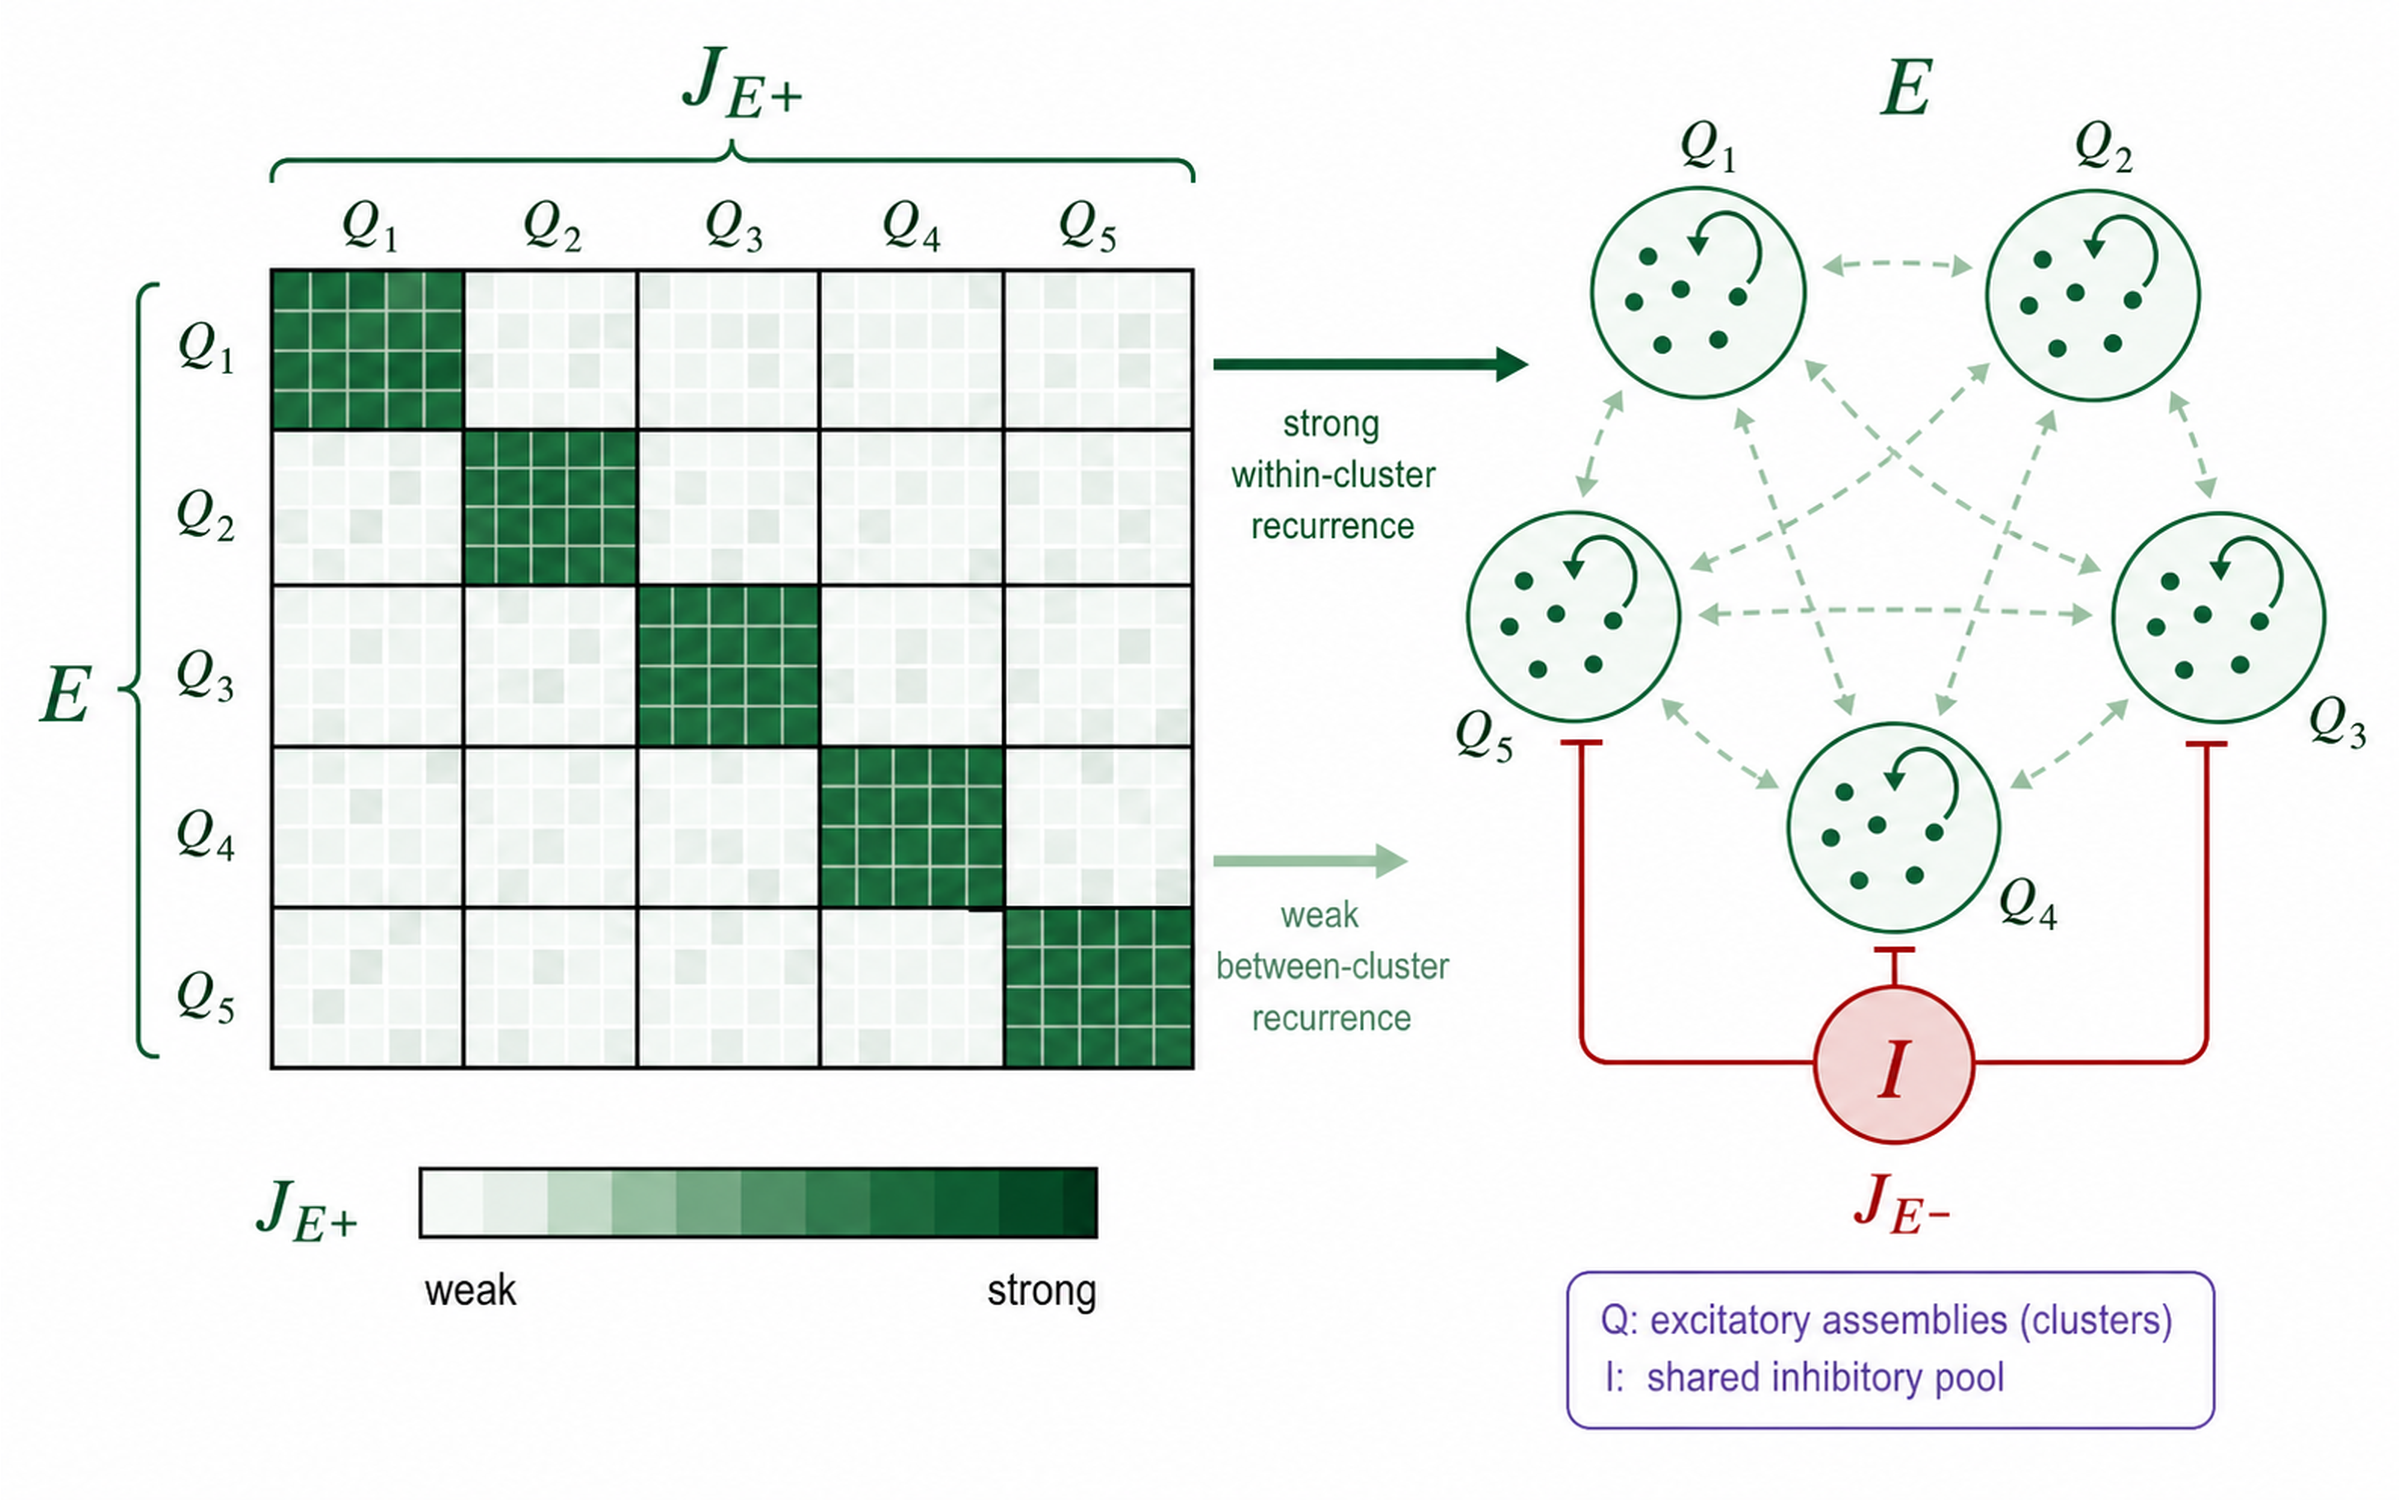
\includegraphics[width=0.72\textwidth]{figures/imagegen/ch05-clustered-connectivity-matrix-img.png}
\caption{Clustered EE connectivity. Diagonal blocks represent potentiated
within-cluster weights $\hat J^{EE}$; off-diagonal blocks represent depressed
between-cluster weights $\check J_{ab}^{EE}$. The block structure turns
assemblies into dynamical units without replacing their neurons by rates.}
\label{fig:ch05-clustered-connectivity-matrix}
\end{figure}

% ============================================================
\section{Active and Inactive Clusters}
\label{sec:active-inactive-clusters}
% ============================================================

Let
%
\begin{equation}
  r_a(t)=\int_{-\infty}^{t}\epsilon(t-t')A_a^E(t')\,dt'
  \label{eq:ch05-filtered-cluster-rate}
\end{equation}
%
be the filtered excitatory activity of cluster $a$. A cluster is called
\emph{active} when $r_a(t)$ lies on a high-rate branch or exceeds a chosen
threshold $r_0$ for a sustained interval. It is \emph{inactive} when it remains
near the low-rate branch. The active-cluster pattern is the set
%
\begin{equation}
  S(t)=\{a\in\{1,\ldots,Q\}: r_a(t)>r_0\}.
  \label{eq:ch05-active-cluster-set}
\end{equation}
%
This set is a coarse macroscopic state. For example, $S=\{1,4\}$ means that
clusters 1 and 4 are active while the others are inactive. The microscopic
state still contains every membrane voltage and every synaptic filter, but the
set $S$ captures the assembly-level configuration.

The reason active clusters can persist is positive feedback. On the filtered
timescale, a high $r_a$ increases the recurrent excitatory input back into
cluster $a$ through $\hat J^{EE}n_E r_a$. At the spike-train level, this is the
same self-excitation term from
\cref{eq:ch05-e-clustered-homogeneous-i-input} after filtering $A_a^E$ by
$\epsilon$. The reason not all clusters simply turn on is competition: shared
inhibition and depressed inter-cluster excitation make simultaneous activation
costly. A schematic input to an excitatory neuron in cluster $a$ is
%
\begin{equation}
  \bar y_a^E
  \approx
  \hat J^{EE}n_E r_a
  +
  \sum_{b\neq a}\check J_{ab}^{EE}n_E r_b
  -
  J^{EI}N_I^{\mathrm{tot}} r_I
  +
  \bar y_E^{\mathrm{ext}},
  \label{eq:ch05-e-cluster-mean-input}
\end{equation}
%
where $r_I$ is the activity of the homogeneous inhibitory pool. The first term
is self-excitation of the assembly, the second term is excitation from other
assemblies, the third term is shared inhibition written with the same
inhibitory-magnitude convention \(J^{EI}>0\), and the final term is external
drive.

% ============================================================
\section{Multistability}
\label{sec:cluster-multistability}
% ============================================================

An attractor is a stable long-term state of the deterministic coarse dynamics.
A clustered attractor network can have many attractors because many subsets of
clusters can be self-consistent. For a particular active set $S$, a mean-field
description asks for rates satisfying
%
\begin{equation}
  r_a
  =
  \phi\!\left(\mu_a(\mathbf r),\sigma_a(\mathbf r)\right),
  \qquad
  a=1,\ldots,Q,
  \label{eq:ch05-cluster-rate-self-consistency}
\end{equation}
%
where $\phi$ is the single-neuron transfer function from
\cref{eq:ch03-transfer-function}, and $\mu_a,\sigma_a$ are the input mean and
fluctuation scale generated by the current vector of cluster rates
$\mathbf r=(r_1,\ldots,r_Q)$. A high-rate solution for $a\in S$ and a low-rate
solution for $a\notin S$ represents an attractor with active set $S$.

Multistability means that more than one such attractor is stable for the same
parameters. The network then has a memory of its history: different initial
conditions or transient inputs can send it to different active-cluster patterns.
This is the attractor-network interpretation of persistent activity and
assembly states.

\begin{figure}[t]
\centering
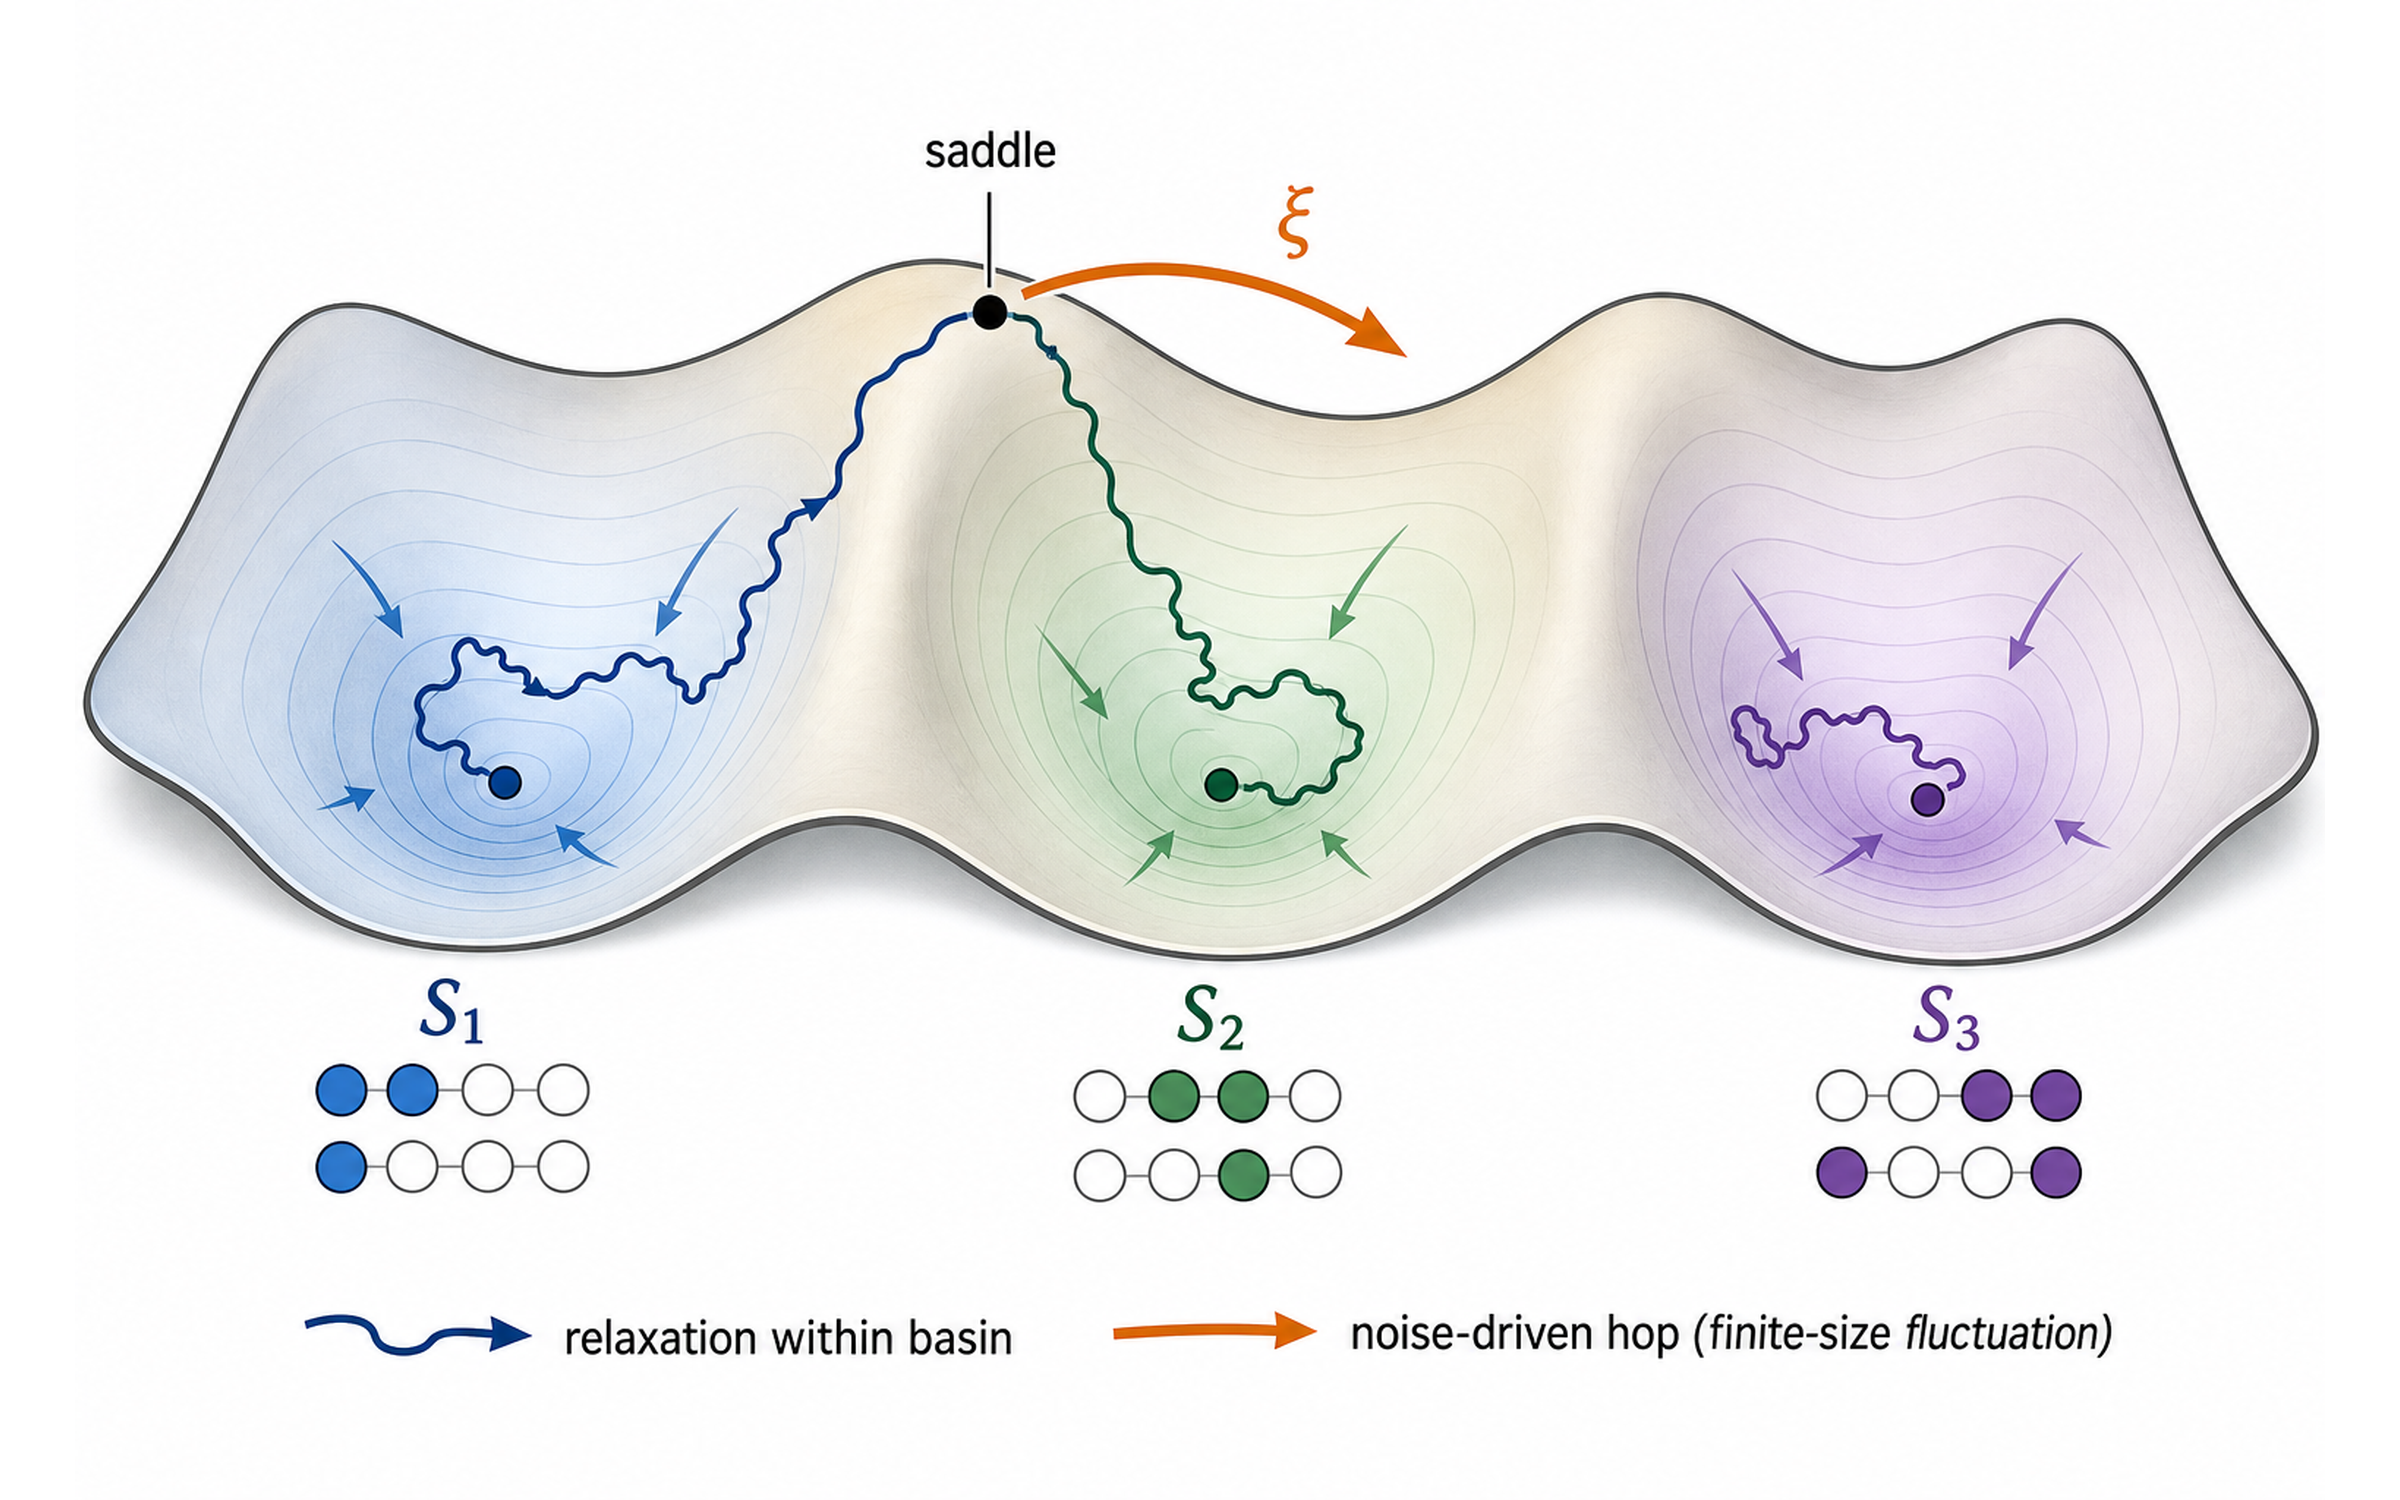
\includegraphics[width=0.90\textwidth]{figures/imagegen/ch05-active-inactive-landscape-img.png}
\caption{Metastable active-cluster patterns. Each basin represents a coarse
state such as $\{1,4\}$ or $\{2,3,5\}$. In an E-clustered network with
homogeneous inhibition, finite-size fluctuations can push the activity across a
saddle, producing switching among attractor-like states.}
\label{fig:ch05-active-inactive-landscape}
\end{figure}

The landscape picture in \cref{fig:ch05-active-inactive-landscape} is only a
cartoon; the true state space is high-dimensional and not generally a gradient
system. Its value is pedagogical. It separates three ideas that are often mixed
together: stable basins, barriers between basins, and noise-driven transitions.

% ============================================================
\section{Metastable Switching and Finite-Size Noise}
\label{sec:finite-size-switching}
% ============================================================

In a finite spiking network, the population activity of a cluster fluctuates
because it averages only finitely many spike trains. If the active excitatory
population in a cluster contains $n_E$ neurons, the baseline finite-size scale is
%
\begin{equation}
  \xi=\frac{1}{\sqrt{n_E}}.
  \label{eq:ch05-xi-finite-size}
\end{equation}
%
This is the same quantity the roadmap sometimes writes as
$\xi=1/\sqrt{N_E^{\mathrm{cluster}}}$, where the superscript here emphasizes
that the count is local to one excitatory cluster, not the total excitatory
population.

When a deterministic attractor is stable but not too deep, fluctuations of size
$\xi$ can occasionally move the network across a basin boundary. The result is
metastability: active-cluster patterns last much longer than the membrane or
synaptic time constants, but they do not last forever.

This finite-size viewpoint predicts a specific scaling. If the number of
clusters is fixed and the number of neurons per cluster grows, then
$\xi\to 0$. Switching caused by finite-size fluctuations should become slower
and may disappear in the infinite-size limit. This is the key interpretation of
E-clustered networks with homogeneous inhibition: their switching can be
valuable for modeling cortical variability, but it is not automatically evidence
for deterministic mesoscopic chaos.
Qualitative trace comparisons in the roadmap's cluster-size notation should
therefore show stronger finite-size switching in smaller clusters, for example
$N_c=107$, than in larger clusters, for example $N_c=250$, when the other
operating parameters are comparable.

\begin{figure}[t]
\centering
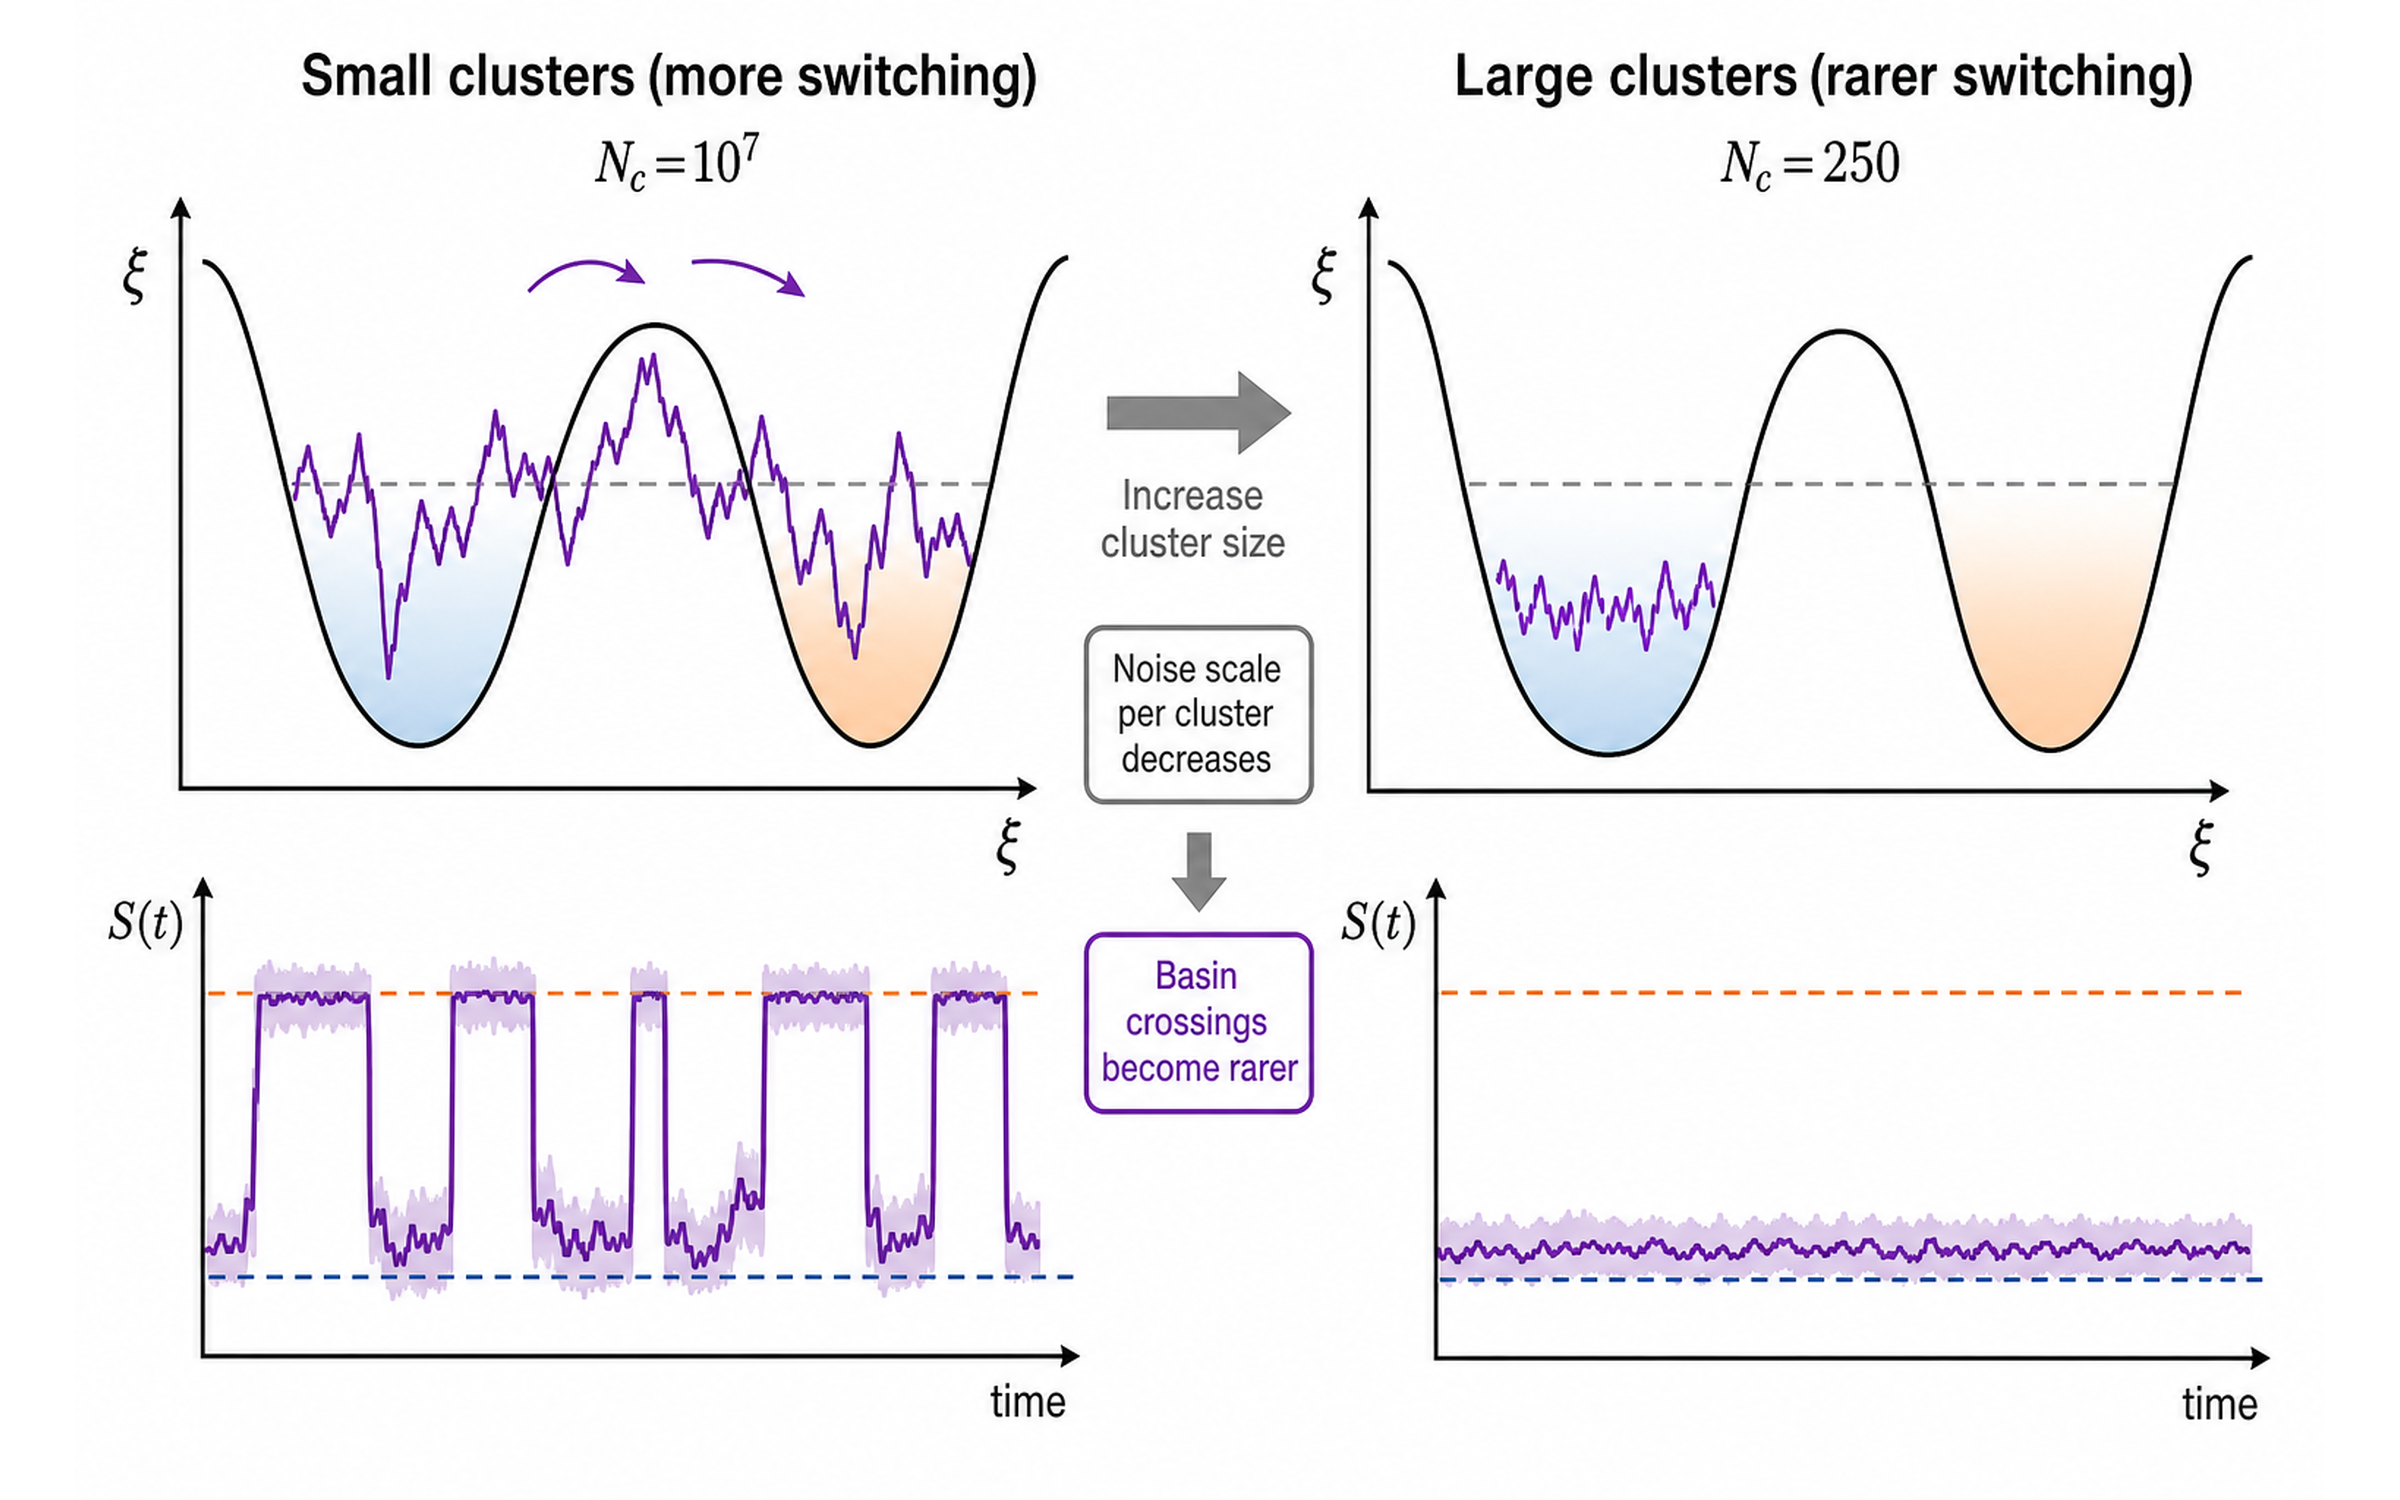
\includegraphics[width=0.92\textwidth]{figures/imagegen/ch05-size-dependent-switching-img.png}
\caption{Finite-size switching prediction. Smaller clusters have larger fluctuation amplitude $\xi=1/\sqrt{n_E}$ and therefore more frequent basin crossings, while larger clusters have smaller finite-size kicks and longer-lived active-set patterns. The comparison is schematic: it isolates the effect of population size at fixed deterministic clustered-network parameters.}
\label{fig:ch05-size-dependent-switching}
\end{figure}

The contrast with later E/I-clustered chapters is now visible. In E-clustered
homogeneous-inhibition networks, the main switching mechanism is finite-size
noise moving among stable attractors. In paired E/I-clustered networks, quenched
inter-cluster variability, later denoted by $\kappa$, can remain effective even
as $\xi\to 0$. Later chapters on paired E/I clusters and diagnostic tests will
turn this contrast into scaling tests.

This also sets up Chapter~6. The mesoscopic object carried forward is the
cluster-rate vector $\mathbf r(t)=(r_1(t),\ldots,r_Q(t))$, or the active set that
this vector defines after separating high-rate from low-rate clusters. In the
present E-clustered picture, irregular switching is finite-size hopping among
deterministic attractors. In the random-rate and SCS-level picture introduced
next, an analogous high-dimensional rate vector can move irregularly under a
deterministic law, so the irregularity can persist even when $\xi\to0$.

\begin{chaptersummary}
\begin{center}
\renewcommand{\arraystretch}{1.45}
\begin{tabularx}{\textwidth}{@{}l X X@{}}
  \toprule
  \textbf{Concept} & \textbf{Equation} & \textbf{Interpretation} \\
  \midrule
  Cluster spike train &
  $s_{a,j}^{\alpha}(t)=\sum_k\delta(t-t_{a,j,k}^{\alpha})$ &
  Microscopic event record inside cluster $a$ \\
  Population activity &
  $A_a^\alpha=n_\alpha^{-1}\sum_j s_{a,j}^\alpha$ &
  Spike train averaged over one cluster population \\
  Clustered input &
  $y_a^\alpha=\sum_\beta\hat J^{\alpha\beta}\sum_j s_{a,j}^\beta+
  \sum_{b\neq a,\beta}\check J_{ab}^{\alpha\beta}\sum_j s_{b,j}^\beta$ &
  Within-cluster and between-cluster sources separated \\
  Mean-preserving EE clustering &
  $\hat J^{EE}+(Q-1)\check J^{EE}=QJ^{EE}$ &
  Potentiation is compensated by inter-cluster depression \\
  Plus/minus factors &
  $J_E^-=(Q_E-J_E^+)/(Q_E-1)$ &
  Dense equal-size clustering preserves the row-average coupling \\
  Active set &
  $S(t)=\{a:r_a(t)>r_0\}$ &
  Coarse state as a set of active assemblies \\
  Finite-size scale &
  $\xi=1/\sqrt{n_E}$ &
  Switching noise decreases as cluster size grows \\
  \bottomrule
\end{tabularx}
\end{center}
\end{chaptersummary}

\begin{conceptquestions}
  \item What dynamical property distinguishes a cell assembly from an arbitrary
  group of neurons?

  \item Why is within-cluster potentiation usually paired with between-cluster
  depression?

  \item In \cref{eq:ch05-e-cluster-mean-input}, identify the term responsible for
  self-excitation and the term responsible for competition among clusters.

  \item What does it mean for an active-cluster pattern $S$ to be an attractor
  of a coarse mean-field description?

  \item Why does finite-size switching predict that transition times should
  increase when $n_E$ grows with the number of clusters fixed?
\end{conceptquestions}
